\documentclass{sig-alternate-2013}

\newfont{\mycrnotice}{ptmr8t at 7pt}
\newfont{\myconfname}{ptmri8t at 7pt}
\let\crnotice\mycrnotice%
\let\confname\myconfname%

\permission{Permission to make digital or hard copies of all or part of this work for personal or classroom use is granted without fee provided that copies are not made or distributed for profit or commercial advantage and that copies bear this notice and the full citation on the first page. Copyrights for components of this work owned by others than ACM must be honored. Abstracting with credit is permitted. To copy otherwise, or republish, to post on servers or to redistribute to lists, requires prior specific permission and/or a fee. Request permissions from permissions@acm.org.}
\conferenceinfo{HotSDN'13,}{August 16, 2013, Hong Kong, China.}
\CopyrightYear{2013} \crdata{978-1-4503-2178-5/13/08}
\clubpenalty=10000
\widowpenalty = 10000 

\newcommand{\superscript}[1]{\ensuremath{^{\textrm{#1}}}}
\def\sharedaffiliation{\end{tabular}\newline\begin{tabular}{c}}

\def\inf{\superscript{*}}
\def\esn{\superscript{\dag}}

\usepackage{listings}
\usepackage{color}
\usepackage{capt-of}

\definecolor{dkgreen}{rgb}{0,0.6,0}
\definecolor{gray}{rgb}{0.5,0.5,0.5}
\definecolor{mauve}{rgb}{0.58,0,0.82}

\lstset{frame=tb,
  language=C++,
  aboveskip=3mm,
  belowskip=3mm,
  showstringspaces=false,
  columns=flexible,
  basicstyle={\small\ttfamily},
  numbers=none,
  numberstyle=\tiny\color{gray},
  keywordstyle=\color{blue},
  commentstyle=\color{dkgreen},
  stringstyle=\color{mauve},
  breaklines=true,
  breakatwhitespace=true
  tabsize=3
}


\pdfpagewidth=8.5in
\pdfpageheight=11in

\begin{document}

\title{Open Transport Switch - A Software Defined Networking Architecture for Transport Networks}

\numberofauthors{6}

\author{
  \alignauthor Abhinava Sadasivarao\inf\\
%  \email{asadasivarao@infinera.com}
%
  \alignauthor Sharfuddin Syed\inf\\
%  \email{ssyed@infinera.com}
%
  \alignauthor Ping Pan\inf\\
%  \email{ppan@infinera.com}
%
\and
  \alignauthor  Chris Liou\inf\\
%  \email{cliou@infinera.com}
%
  \alignauthor Andrew Lake\esn\\
% \email{alake@es.net}
%
  \alignauthor  Chin Guok\esn\\
%  \email{chin@es.net}
%
\and
  \alignauthor \\
%
  \alignauthor Inder Monga\esn\\
%  \email{inder@es.net}
%
  \alignauthor \\
  \sharedaffiliation
  \begin{tabular}{ccc}
    \affaddr{{\inf}Infinera Corporation{\ }} & & \affaddr{{\esn}Energy Sciences Network{\ }} \\
%    \affaddr{169 W Java Dr}                         & & \affaddr{Lawrence Berkeley National Laboratories}\\
    \affaddr{Sunnyvale, CA 94089}              & & \affaddr{Berkeley, CA 94720}\\
    \affaddr{\{asadasivarao, ssyed, ppan, cliou\}@infinera.com} & & \affaddr{\{andy, chin, inder\}@es.net}\\
  \end{tabular}
}
\maketitle
\begin{abstract}
There have been a lot of proposals to unify the control and management of packet and circuit networks but none have been deployed widely. In this paper, we propose a simple programmable architecture that abstracts a core transport node into a programmable virtual switch, that meshes well with the software-defined network paradigm while leveraging the OpenFlow protocol for control. A demonstration use-case of an OpenFlow-enabled optical virtual switch implementation managing a small optical transport network for big-data applications is described. With appropriate extensions to OpenFlow, we discuss how the programmability and flexibility SDN brings to packet-optical backbone networks will be substantial in solving some of the complex multi-vendor, multi-layer, multi-domain issues service providers face today.
\end{abstract}

\category{C.2.1}{Computer-Communication Networks}{Network Architecture and Design}[Circuit-switching networks]
\category{C.2.3}{Computer-Communication Networks}{Network Operations}[Network management] 

\terms{Design, Standardization}

\keywords{sdn; transport networks; optical networks; virtualization; otn}

\vfill\eject
	
	\section{Introduction}
	Significant advances in optical technologies, bit rates and deployment of Optical Transport Network (OTN) \cite{otn} protocols have enabled transport networks to provide flexible 
	multiplexing and switching functions in addition to basic data transport and survivability. In addition, transport network elements are  being supplemented with more intelligent 
	set of features for flexible management. The growth in traffic volumes, changing traffic profiles and types of applications has prompted service providers to rethink not only how to
	engineer their IP and optical backbone transport optimally, but also to ease their operational and management overhead.\\
	
	In the Internet core, traditionally, the design approach has been to place all the network functions within the IP layer
	(routing, signaling, protection) and use static optical trunks interconnecting these L2/L3 devices. This hop-by-hop architecture of packet processing
	and forwarding can be optimized significantly by taking advantage of the dynamic transport capabilities offered by the state-of-the-art optical network. 
	In addition, service providers typically manage their L3 networks and transport layer operations independently. \\
	
	In this multi-layer setup, provisioning bandwidth involves multiple steps: provisioning transport circuits, configuring interfaces and creating appropriate forwarding entries in the L3 devices, and in the end, bridging the 	path to create an end-to-end circuit. The distributed nature of the provisioning requires UNI and NNI signaling to help provision each segment of the actual datapath. This approach adds complexities to the transport 	control plane mechanisms (GMPLS \cite{gmpls}/MPLS \cite{mpls}/MPLS-TP \cite{mpls-tp}). \\

	The latest trends in application delivery architectures, like cloud computing, not only aggregate the user traffic but also create large data flows between consolidated data-centers for state and data synchronization. The 	need for cost and performance optimization including the need for service providers to create new network services relevant to the above application patterns is driving the requirements for dynamic, multi-layer, multi-domain networking. Multi-layer optimization, with applications such as dynamic router bypass, not only has technology drivers, but also influences CapEx economics. Even though the benefits of such approaches are well understood as well as protocols have been created by the community - the complexity of existing protocols, vendor  interoperability and lack of management tools has prevented these applications from being deployed.\\
	
	Software-Defined Networking (SDN), decoupling of the data plane from control plane, has been discussed recently \cite{Das2012} 
	as a viable and simple approach to provide the required functionality. The approach promises meeting the manageability, flexibility, and evolvability 
	requirements in large service provider networks. Although, much of SDN efforts today are concentrated on networks at Layer 2 and above. Many vendors have
	added OpenFlow capabilities to their Gigabit Ethernet switches. There have also been efforts in building
	hardware architectures \cite{Mogul2012} and switch fabrics for efficient OpenFlow enabled network devices
	\cite{Casado2012}. OpenFlow based enterprise wireless network management has also been proposed \cite{Suresh2012}. All these are Ethernet/IP centric.\\
	
	In this paper we propose a virtual abstraction of the transport element, Open Transport Switch (OTS), that integrates within a SDN framework and
	offers simple OpenFlow protocol based control of the packet-optical cross-connect (XCON) and bandwidth allocation capability of the optical element. In addition,
	we showcase a prototype implementation of this abstraction and deployment at a test network in Long Island. We show SDN as a
	viable approach for building wide-area packet-optical networks. 

\iffalse
	The growth in traffic volumes and types has prompted service providers to rethink not only how to
	engineer their IP and optical backbone transport, but also to ease operational and management overhead.
	In the core, traditionally, the approach has been to place all the network functions within the IP layer
	(routing, signaling, protection) and use dumb optical trunks interconnecting these L2/L3 devices.
	Therefore, a significant amount of service providers' investments are in the underlying transport
	infrastructure. This optical transport layer offers high-capacity links which typically allows tens of
	gigabits of traffic to be transported in a point-to-point fashion. Given the increasing bandwidth
	demands, the shift is towards deploying 100Gbps per wavelength in the long haul backbone, with a gradual
	transition to a converged packet-optical core. \\
			
	Due to the increased capacity, transport network elements are being supplemented with more intelligent
	set of features for easier management. Service providers typically manage their L3 networks and transport
	layer operations independently. In this multi-layer setup, provisioning bandwidth involves multiple
	steps: creating necessary interfaces and forwarding entries in the L3 devices and provisioning circuits
	in the transport networks, closing the end-to-end path. Given the distributed nature of the protocols,
	various UNI and NNI signaling needs to happen before the actual datapath is complete. This is adding
	complexities to the transport control plane mechanisms (GMPLS \cite{gmpls}/MPLS \cite{mpls}/MPLS-TP
	\cite{mpls-tp}). It becomes crucial to have flexibility, programmability and automated control from an
	OAM\&P and FCAPS perspective. Multi-layer optimization is not just technical, but an economical issue
	too. \\
		
	Software Defined Networking (SDN) decouples data plane from control plane. This promises the necessary
	manageability, flexibility and evolvability that is required in large service provider networks.
	Although, much of SDN efforts today are concentrated on networks at Layer 2 and above. Many vendors have
	added OpenFlow capabilities to their Gigabit Ethernet switches. There have also been efforts in building
	hardware architectures \cite{Mogul2012} and switch fabrics for efficient OpenFlow enabled network devices
	\cite{Casado2012}. Not just WANs, SDN has been making inroads into LANs also. OpenFlow based enterprise
	wireless network management has also been proposed \cite{Suresh2012}. All these are Ethernet/IP centric.
	Echoing a similar philosophy, many of the SDN ideas can be extended to optical transport networks too.
\fi
\section{Architecture}
\label{sec:arch}
	The central approach is to \emph{abstract} the interface between packet and circuit layers, leading to \emph{virtualization}
	of the transport layer. Let us consider a typical multi-layer service provider network (Fig. \ref{fig:MDL}). The network is segmented into
	various layers each running their own control plane for routing and signaling. Each layer may have equipment from different vendors. Multi-layer
	integration becomes a challenge as 1) GMPLS protocols for multi-layer require UNI relationship which hides each layer's topology (Fig. \ref{fig:MLwoOF})
	2) Multi-vendor implementations of GMPLS protocols and path-finding are fairly different with interoperability at a least common denominator of functionality 
	3) Different EMS/NMS systems are ultimately used to manually manage each vendor, leading to a static, pre-planned network solution. \\

\begin{figure}[htb]
	\centering
	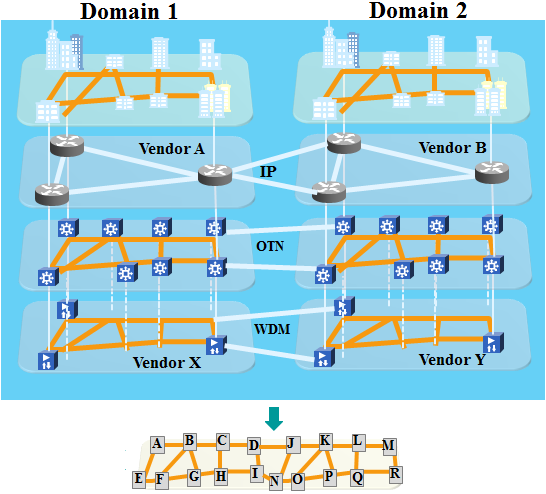
\includegraphics[scale=0.50]{MultiDomainLayer.png}
	\caption{Multi-Domain, Multi-Layer}
	\label{fig:MDL}
	\end{figure}
	
	On the other hand, the applications at the edges of these networks require high-bandwidth paths for exchange of data, for example data center interconnects.
	These connections require connectivity and varying amounts of bandwidth, irrespective of the protocols used to transport the information. The underlying
	transport infrastructure could be packet/MPLS, OTN or MPLS-TP. If the resources viz. ports, links and bandwidth can be virtualized with generic abstractions, 
	the applications would need to program this \emph{\bf virtual overlay network} of devices interconnected by links (Fig. \ref{fig:MDL}). The network then truly becomes open, 
	programmable and flexible. \\
		
	\begin{figure}[htb]
	\centering
	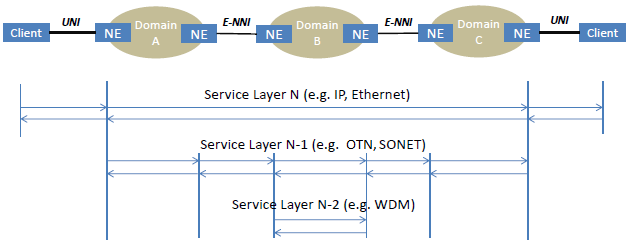
\includegraphics[scale=0.50]{MLwoOF.png}
	\caption{Service Provider Transport Network}
	\label{fig:MLwoOF}
	\end{figure}

	\textit{Open Transport Switch (OTS)} is an OpenFlow \cite{OF1.0} enabled light weight, virtual switch
	that represents a transport network element (NE).  Applications can now use the northbound API of a SDN controller to request
	provisioning of circuit cross-connects or aggregation of packet interfaces into optical trunks with the required
	capacity and QoS parameters, if needed. This gives service providers the ability to create a unified view  of the
	network (Fig. \ref{fig:MLwOF}).		
	The SDN Controller offers the abstract topology to smart applications enabling them to perform optimal path computation,
	provisioning and monitoring based on their constraints. Applications not capable or interested in their own path-computation can request the
	bandwidth capacity and QoS, outsourcing the end-to-end path computation to a specialized carrier SDN controller or leverage an application similar to PCE, 
	that can match the request for the end-to-end path across 	multiple domains/layers to meet the requested SLA. 

\iffalse
	The main idea here is \emph{virtualization} and \emph{abstraction}: how various entities in the network could 
	be virtualized into nodes/links/bandwidth and how to abstract these resources to give programmability.
	Let us consider the common scenario found in service provider networks. The network is segmented into
	various layers each running their own control plane for routing and signaling (Fig. \ref{fig:MLwoOF}).
	These L1/L2/L3 equipments may all possibly be sold by different vendors. Multi-layer integration becomes
	a challenge and service provider now has to use multiple EMS/NMS to manage the entire network. The
	interaction between these protocols at different layers introduces other intricacies such as graceful
	failure propagation. If there is a fiber cut (Layer 1), the devices need to appropriately raise alarms to
	notify the edge devices on the upper layers (L2/L3). \\

\begin{figure}[htb]
	\centering
	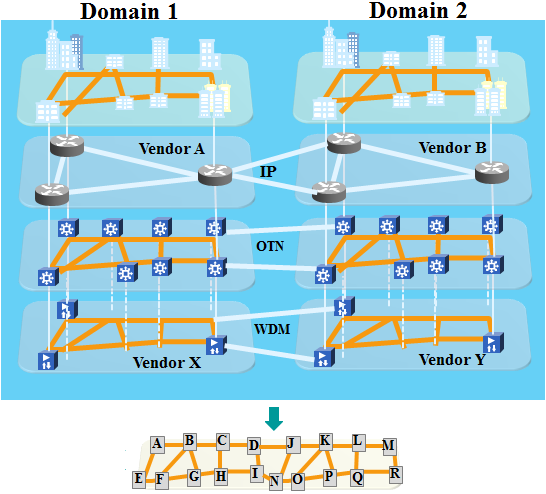
\includegraphics[scale=0.50]{MultiDomainLayer.png}
	\caption{Multi-Domain, Multi-Layer}
	\label{fig:MDL}
	\end{figure}
	
	Applications at the edges of these networks require datapath for exchange of data. For example, consider data
	center interconnects; Large amounts of data need to be exchanged between data centers. These data center
	applications require connectivity and bandwidth irrespective of the technology that is used to enable
	them. The underlying transport infrastructure could be IP, Packet/MPLS or Optical. If the resources viz.
	ports, links and bandwidth can be virtualized with generic abstractions, all the applications would need
	is to program this \emph{\bf virtual overlay network} of devices interconnected by links (Fig.
	\ref{fig:MDL}). The network truly becomes open, programmable and flexible. \\
		
	\begin{figure}[htb]
	\centering
	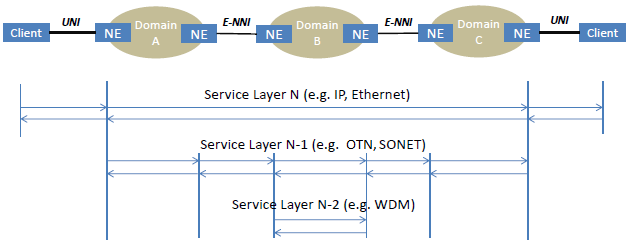
\includegraphics[scale=0.50]{MLwoOF.png}
	\caption{Service Provider Transport Network}
	\label{fig:MLwoOF}
	\end{figure}

	\textit{Open Transport Switch (OTS)} is an OpenFlow \cite{OF1.0} enabled light weight, virtual switch
	that manages a transport network element (NE). With a controller, the transport domain now could be
	controlled via SDN. Applications can now talk to the controller to request provision trunks of required
	capacity with additional QoS parameters if any. This gives service providers a unified view and of the
	network (Fig. \ref{fig:MLwOF}). This also greatly simplifies the control plane to manage NEs at multiple
	layers. The SDN Controller can interface with smart applications to perform path computation,
	provisioning and monitoring. The application requesting the bandwidth will only be concerned about the
	capacity and QoS guarantees. It is up to the controller (or the application talking to the controller) to
	find an end-to-end path going over multiple domains/layers, meeting the SLA.
\fi
	\begin{figure}[htb]
	\centering
	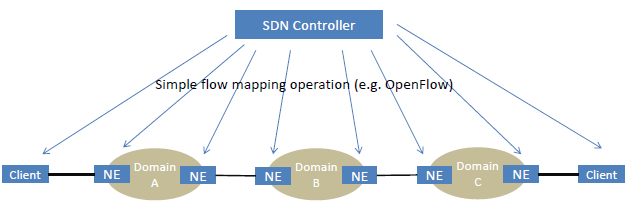
\includegraphics[scale=0.50]{MLwOF.png}
	\caption{SDN Enabled Transport Network}
	\label{fig:MLwOF}
	\end{figure}

	Fig. \ref{fig:OTSArch} shows the building blocks of OTS consisting of the following components:

	\textit{Discovery Agent}: is responsible for discovery and registration of SDN-controlled resources. 
		It appropriately notifies the Controller dynamically as and when the NE and/or the Network state changes 
		(for example, link up/down). This typically happens via the switch
		\texttt{OFPT\_FEATURES\_REQUEST}, \texttt{OFPT\_FEATURES\_REPLY} and
		other related \texttt{Modify State} messages \cite{OF1.0}. How the discovery agent retrieves this
		information from the NE is upto the implementation or via proprietary vendor interfaces. \\

	\textit{Control Agent}: is responsible for monitoring and propagating notifications and alarms to the
		Controller, allowing network admins to monitor performance, faults and alarms in the network. 
		These include change notifications for any new equipment/facilities provisioned/deprovisioned. Loss-of-light, Loss-of-sync, Loss-of-signal are some 
		examples of alarms. Faults could range from link failures to equipment failures. (Note that some of
		equipment related alarms could be reported by both the Control and Discovery agents). This way, the
		controller's state is asynchronously (or synchronously) kept consistent with the state of the underlying
		network. \\

	\textit{Dataplane Agent}: is responsible to program the NE datapath to create/update/release
		circuits/LSP. The datapath entities could be Time slots, XCONs or MPLS labels. This
		programs the underlying network infrastructure and helps complete the datapath. The controller sends
		appropriate OpenFlow messages (similar to \texttt{OFPT\_FLOW\_MOD} message). Again, how the Dataplane
		Agent programs the particular NE database/forwarding tables could be through vendor specific interfaces. \\
	
	The northbound interface from OTS to the Controller is OpenFlow 1.0 \cite{OF1.0}. Given that OTS is
	virtualizing transport NE, much of the Ethernet centric OpenFlow messages are not used. With addition of
	extensions (see sections \ref{sec:ofext} \& \ref{sec:design}), the Controller can send requests to OTS
	to provision/release transport circuits.
	
	OTS being a virtual switch has multiple advantages:

	\begin{itemize} 
	   \item OTS is minimally stateful: All the alarms, stat counters, forwarding table entries are 
		stored in the NE database and could be retrieved on-demand. OTS need not maintain these managed objects. 
		This enables OTS to be light on the use of on-switch resources.
	   \item OTS is lightweight and portable: Given that most of the state is maintained by the NE, if the southbound 
		interface from the OTS agent to the NE is flexible to be implementation and/or vendor specific, the OTS 
		abstraction could be made to run recursively on a standalone server or EMS or any other machine which can communicate 
		and maintain an active OpenFlow session with the Controller.
	   \item OTS Southbound Interface: The southbound interface from the OTS agent to the NE could also be 
		standard hardware abstraction layer allowing plug and play of multi-vendor transport elements that conform to that interface. 
  	   \item Multiple OTS agents could be run on the same NE. These different instances can be used to hard-partition the ports/wavelengths 
	   present on the NE and manage their respective resources only, thus supporting a multi-tenant architecture. 
		(See section \ref{sec:otvs})
	\end{itemize}


	\begin{figure}[htb]
	\centering
	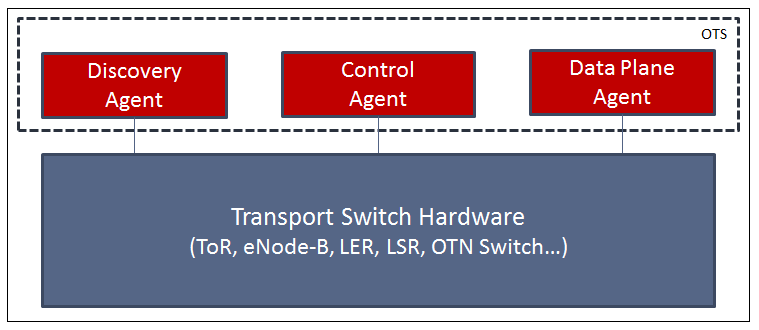
\includegraphics[scale=0.37]{OTSArch.png}
	\caption{OTS Building Blocks}
	\label{fig:OTSArch}
	\end{figure}

	\subsection{OpenFlow Extensions}
	\label{sec:ofext}
	
	OpenFlow \cite{OF1.0} only addresses packets, thus is L2/L3 centric as of today. With the need to control optical transport
	equipment with the same software controller, the protocol currently needs to incorporate circuit switching constructs like time-slots or
	cross-connects. We propose extending OpenFlow with messages that enable provisioning/release of
	circuits. In order to virtualize the network, we use opaque, MPLS-style labels to represent links i.e. a sequence of ingress/egress ports. We also indicate the style of circuit that needs to be setup (see
	section \ref{sec:modes}). Along with these, the message includes service rate and latency parameters along
	with provisioning actions (\texttt{ADD\_XCON} and \texttt{REM\_XCON}). For now, we assume the type of service/traffic 
	to be Ethernet. However, the protocol could be extended to OC-192, OTU3, Fibre Channel and so on.


	\begin{lstlisting}
struct ofp_id {
	// Host ID - DCN IP Address of the Node
	uint32_t node;

	// Flow ID maintained by the Controller
	uint32_t label;
};

struct ofp_xconn {
	struct ofp_header header; // OFPT_VENDOR
	uint32_t vendor;  // Vendor ID

	uint8_t pad[4];
		  
	struct ofp_id src; // Source of the flow
	struct ofp_id dst; // Destination of the flow
		   
	uint32_t rate;     // Rate of service (Mbps)
	uint8_t latency; // Latency - 0 to 255
	uint8_t style;     // Implicit = 1 Explicit = 2

	// Unidirectional = 1 Bidirectional = 2
	uint8_t directional;

	uint8_t pad_extra[1];

	// ADD_XCONN = 0xFF REM_XCONN = 0xFE
	struct ofp_action_header actions[0];
};
OFP_ASSERT(sizeof(struct ofp_xconn) == 40);
	\end{lstlisting}

	\vfill\eject
	\subsection{Modes of Operation} \label{sec:modes}
	We already described how SDN for transport can provide an alternative to inter-working UNI/NNI 
	protocols associated with distributed routing and signaling. Integrating OTS into today's large service provider transport
	networks may become a very complex exercise (we are infact trying to make transport networks more
	flexible and manageable!). Taking this into account, we propose two modes of operation to allow smooth
	integration of, and transition to transport SDN.

	\begin{figure}[htb]
	\centering
	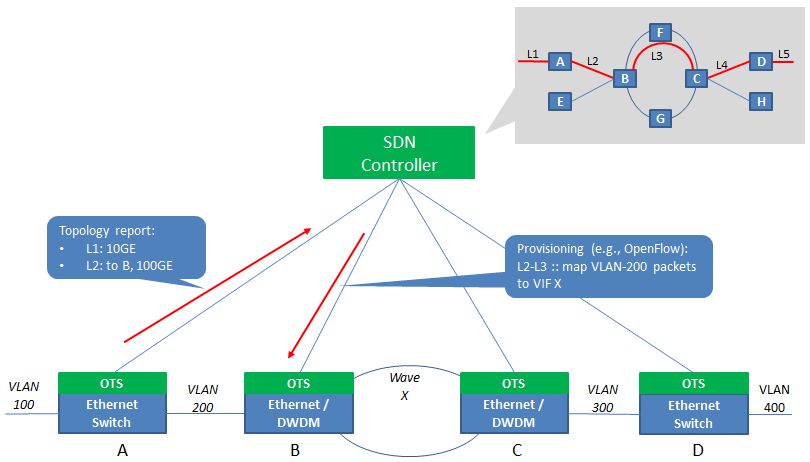
\includegraphics[scale=0.37]{OTSExplicit.png}
	\caption{Transport SDN Explicit Mode}
	\label{fig:OTSExplicit}
	\end{figure}


 \subsubsection{Explicit Mode}
 Fig. \ref{fig:OTSExplicit} depicts \textit{Explicit Mode}. In this mode, the Controller has the knowledge
 of every NE in a particular domain. After optimal/constrained path computation, provisioning a circuit becomes a
 exercise of the Controller programming all the transport devices along the path in a hop-by-hop
 manner across single or multiple transport domains.
 
 \subsubsection{Implicit Mode} Fig. \ref{fig:OTSImplicit} depicts \textit{Implicit Mode}. In this mode,
 the Controller is aware of only the edge nodes in every transport domain (Ethernet/MPLS/OTN). Within the
 domain, the existing routing and signaling control plane can be used to setup path. The
 Controller sends provisioning request, specifying the source and destination to the SDN-aware nodes
 at the edges of the network. The source node then triggers MPLS/GMPLS control plane to setup the circuit.
 The Controller being aware of NE type and capabilities, \textit{stitches} these segments across multiple
 domains to form an end-to-end circuit. Implicit mode adds great flexibility in gradually incorporating
 OTS architecture into existing transport networks. Without disrupting current deployments, service
 providers may choose to continue using intra-domain control plane while still being SDN aware. From a
 Controller's perspective, this edge-to-edge intra-domain path appears as a single network fabric of a
 given capacity. Service providers depending on the necessary management effort, can gradually make
 all the NEs SDN capable, moving to an explicit deployment model.\\

 \begin{figure}[htb]
 \centering
 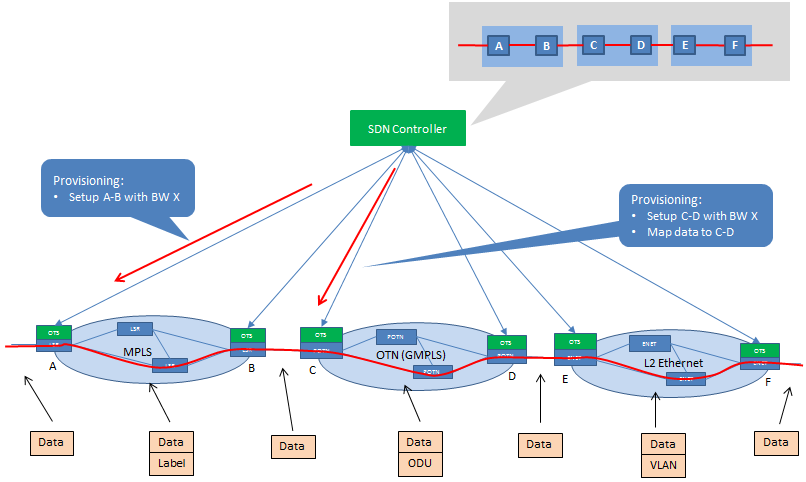
\includegraphics[scale=0.37]{OTSImplicit.png}
 \caption{Transport SDN Implicit Mode}
 \label{fig:OTSImplicit}
 \end{figure}

 Note that these are not the only two feasible models in Transport SDN. In a given network, it is possible to have
 SDN circuits created with mix of implicit and explicit modes. This prototype demonstrates the larger concept.

\vfill\eject
\section{Implementation}
\label{sec:design}
 Section \ref{sec:arch} described the building blocks of OTS. The prototype OTS implementation only has the 
 Dataplane agent functionality built in. Rest of the subsystems will be integrated in the future. 

 \subsection{Controller}
 \label{sec:oscars}
 \textit{On-Demand Secure Circuits and Advanced Reservation System} (OSCARS) \cite{Guok2008} is a provisioning system developed by Energy Sciences Network (ESnet). 
 It provides multi-domain, high-bandwidth, virtual circuits that guarantee end-to-end network data transfer performance. Today, OSCARS virtual circuits carry about fifty 
 percent of ESnet's annual 60 petabytes of traffic, supporting large scale sciences such as High Energy Physics, Climate, Computational Astrophysics, and Biological and Environmental Research.\\
 
 The OSCARS system in this instance acts as a typical SDN controller, albeit with several specific extensions (see \ref{sec:ofext}) to leverage the transport OpenFlow capabilities 
 of the OTS.  The initial handshake between OSCARS and OTS involves the characteristic exchange of \texttt{OFPT\_HELLO} followed by \texttt{OFPT\_FEATURES\_REQUEST} and 
 \texttt{OFPT\_FEATURES\_REPLY} messages \cite{OF1.0}. However, OpenFlow extension messages as described above are used for optical specific information.
 
 \subsection{OTS Agent - Virtual Switch}
 \label{sec:otvs}
 
 The prototype OTS implementation is coupled with the Infinera DTN \cite{DTN}, which embodies the optical transport NE.  The DTN has fully
 flexible OTN, SONET/SDH and Ethernet add/drop capabilities with OTN \cite{otn} line side wavelength Optical Carrier Groups (OCG), and includes an 
 embedded GMPLS control plane for end-to-end routing and provisioning. \\
 
 To determine the tributary ports and line-side wavelengths to be used, a simple manually edited configuration file is referenced. In the future, this will be part of automated topology learning and could also be managed by OF-Config set of protocols.  Given that
 these are TDM circuits, the incoming traffic payload is digitally wrapped/containerized into OTN optical channels and transported.  
 There is no header or label lookup done on incoming traffic, and therefore the configuration  file itself is sufficient as a simple flow table. 
 In addition, the configuration file can specify "slices" of an NE that can be virtualized into separate tributary port/line side wavelength 
 resources controlled by distinct OTS instances.  This allows service providers to sell wholesale bandwidth to multiple third party/tier-2 providers,
 who can only control their portion of the equipment/resources.

\section{Results and Observations}
\label{sec:results}
 \subsection{Network Setup}
 \label{sec:testbed}
 We used ESnet's Long Island Metropolitan Area Network (LIMAN) to demonstrate SDN control of the
 transport optical backbone by combination of OSCARS controller and OTS. Fig. \ref{fig:LIMAN} shows the setup. DTN nodes 
 A and B are SDN aware and the two embedded OTS agents offer an abstracted view of the NEs. These nodes connect
 to the ESnet production network via pair of optical fibers lit via a DWDM system. These nodes are interconnected by a direct
 fiber connection as well. Hosts, each with 40G Ethernet interfaces, connect to each of these transport SDN nodes. Using OpenFlow,
 we setup two 40G circuits between the nodes A and B, one circuit over the direct fiber link and the other over the set of production nodes.
 The fiber path traversed by the optical circuit is transparent to the end-hosts. The hosts see each circuit as a direct one-hop IP link connecting each other.

	\begin{figure}[htb]
	\centering
	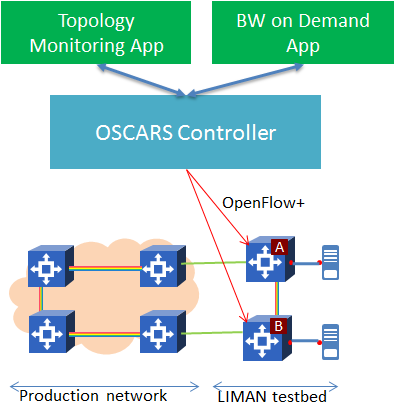
\includegraphics[scale=0.50]{LIMAN.png}
	\caption{Network Setup}
	\label{fig:LIMAN}
	\end{figure}

 \subsection{Measurements}
 \label{sec:measure}
 The measurements were done for a 40GbE circuit reservation from Node A to B (Fig. \ref{fig:LIMAN}). This only includes the time 
 taken by the Controller to compute the path.
 The time can be further optimized, by leveraging faster processing platforms for the Controller. This metric was specifically chosen so we could compare the
 time involved in setting up the path using SDN Controller and contrast it with a distributed signaling approach. We take note that the time to configure each NE to setup a circuit remains the same 
 irrespective of the centralized SDN or distributed signaling approach taken to communicate the cross-connect action.

 \begin{center}
  \begin{tabular} { | c |  c | c | c | c | }
   \hline
    Mode & Min & Max & Mean & Std. Dev \\ \hline
    Implicit & 2   &   7    & 2.84  & 0.98 \\
    Explicit & 2   &   5    & 2.95  & 0.87 \\
   \hline
  \end{tabular}
  \captionof{table}{Circuit path computation latencies (s)}
  \label{tab:measurements}
 \end{center}

 Given a fairly simple topology, higher latency observed is for the first circuit setup request. For the first request, OpenFlow session needs
 to be established with the OTS agents and hence the higher latency. Once the session is active, the time delay just involves the
 Controller computing the required path based on the existing topology. Since this experiment is a prototype, most of the topology
 and node/link information was statically configured. In the future, OTS Discovery agent is responsible to provide the Controller with the
 necessary topology and network resource information. This will be planned within the next phase of work.

\section{Scope for Future Work}
 \label{sec:future}
  There are several additions to OTS that could provide full featured network virtualization capabilities. From an
  implementation perspective, we wish to fully integrate the Monitoring and the Discovery agents into
  OTS for fault/alarm propagation and port/link discovery respectively. Currently for this prototype implementation, the ports, optical 
  channels and links are hand-configured through a configuration file.
  But we would need a dedicated info model, similar to Open vSwitch Database \cite{ovsdb}, to house
  the configuration information and advertise it to the Controller. This allows the Controller to discover
  the complete topology depending on the mode of operation (Implicit/Explicit). JSON encoded data 
  could be used to exchange the extracted topology between OTS and the Controller. \\

  From the point of view of standardization, other important functions that are inherent to core transport networks
  have to be factored in, for example, protection and restoration. Typically, these are part of the
  control plane (MPLS FRR or GMPLS restoration).Thorough studies need to be done to determine if
  these require explicit incorporation within OpenFlow protocol, or the embedded software layer on the transport NE can take care
  of that function. Further, if domain specific parameters (like optical impairments, OSNR, channel power levels etc)
  are needed, these need not be a part of the protocol itself. Instead, a management interface like OF-Config or
  NETCONF can be used to manage these.

\section{Conclusion}
 The SDN approach has been applied successfully to the optical transport network through the instantiation of a virtual transport switch architecture and abstraction described in this paper.
 This approach has been shown as practical through implementation and demonstration over a metro-area network. This architecture can easily be extended from optical transport to converged packet-optical transport  architectures including MPLS or MPLS-TP core backbones as well. Including the transport network within the SDN paradigm provides compelling technical and economic advantages to large service providers looking to efficiently engineer, manage and evolve their networks to meet the 'big data' challenges and cater to new on-demand 'cloud' applications. The transport infrastructure can now be made open and uniformly programmable, enabling multi-layer, multi-domain and multi-vendor optimization in both core and metro networks.\\

 Network virtualization through OTS enables building an overlay network that applications can program to  meet their specific service requirements irrespective of underlying protocol or encapsulation layers (L1/L2/L3 or OTN/MPLS/IP) used. Efforts are already underway within Open Networking Foundation (ONF) to build consensus around the standardization of transport extensions to OpenFlow (Optical Transport WG). We believe that these extensions will be an important  element in control and management of packet-optical architectures within the core of the network.

\bibliographystyle{acm}
%\bibliography{ots} 

\begin{thebibliography}{10}

\bibitem{Casado2012}
{\sc Casado, M., Koponen, T., Shenker, S., and Tootoonchian, A.}
\newblock {Fabric: a retrospective on evolving SDN}.
\newblock In {\em {Proc. of HotSDN}\/} (2012).

\bibitem{Das2012}
{\sc Das, S., Parulkar, G., and McKeown, N.}
\newblock {SDN Based Unified Control Architecture}.
\newblock In {\em Photonics Conference (IPC), 2012 IEEE\/} (2012),
  pp.~778--779.

\bibitem{Guok2008}
{\sc Guok, C., Robertson, D., Chaniotakisy, E., Thompson, M., Johnston, W., and
  Tierney, B.}
\newblock {A User Driven Dynamic Circuit Network Implementation}.
\newblock In {\em GLOBECOM Workshops, 2008 IEEE\/} (2008), pp.~1--5.

\vfill\eject
\bibitem{mpls}
{\sc IETF}.
\newblock {RFC3031: Multiprotocol Label Switching Architecture}, January 2001.

\bibitem{gmpls}
{\sc IETF}.
\newblock {Generalized Multi-Protocol Label Switching (GMPLS) Architecture},
  July 2004.

\bibitem{mpls-tp}
{\sc IETF}.
\newblock {RFC6215: A Framework for MPLS in Transport Networks}, July 2010.

\bibitem{ovsdb}
{\sc IETF}.
\newblock {ovsdb-draft-00: The Open vSwitch Database Management Protocol},
  August 2012.

\bibitem{DTN}
{\sc {Infinera}}.
\newblock {DTN} http://www.infinera.com/products/dtn.html.

\bibitem{otn}
{\sc {ITU}}.
\newblock {G.709: Interfaces for Optical Transport Network}, Feb 2012.

\bibitem{Mogul2012}
{\sc Mogul, J.~C., and Congdon, P.}
\newblock {Hey, you darned counters!: get off my ASIC!}
\newblock In {\em {Proc. of HotSDN}\/} (2012).

\bibitem{OF1.0}
{\sc Pfaff, B.}
\newblock {OpenFlow Switch Specifications 1.0.0}, Dec 2009.

\bibitem{Suresh2012}
{\sc Suresh, L., Schulz-Zander, J., Merz, R., Feldmann, A., and Vazao, T.}
\newblock {Towards programmable enterprise WLANS with Odin}.
\newblock In {\em {Proc. of HotSDN}\/} (2012).

\end{thebibliography}

\end{document}